% arara: xelatex
\documentclass[tikz]{standalone}

% Copy of relevant parts from the main preamble.
\usepackage{mathtools}

% Uncomment the following to use Times New Roman and Cambria Math
% \usepackage{unicode-math}
% \unimathsetup{math-style=TeX}
% \setmathfont[range=\mathup/{num}]{Times New Roman}
% \setmathfont[range=\mathit/{greek,Greek,latin,Latin}]{Cambria Math}
% \setmathfont[range=\mathup/{greek,Greek,latin,Latin}]{Cambria Math}
% \setmathfont[range={"2212,"002B,"003D,"0028,"0029,"005B,"005D,"221A,
% "2211,"2248,"222B,"007C,"2026,"2202,"00D7,"0302,"2261,"0025,"22C5,
% "00B1,"2194,"21D4,"2032}]
% {Cambria Math}
% \setmainfont[Ligatures=TeX]{Times New Roman}

% Uncomment the following to use Linux Libertine
% \usepackage[libertine]{newtxmath}
% \usepackage[no-math]{fontspec}
% \setmainfont{Linux Libertine O}

% Uncomment the following to use TeX Gyre Termes
% \usepackage{unicode-math}
% \unimathsetup{math-style=TeX}
% \setmainfont{TeX Gyre Termes}
% \setmathfont{TeX Gyre Termes Math}

% Uncomment the following to use TeX Gyre Pagella
\usepackage{unicode-math}
\unimathsetup{math-style=TeX}
\setmainfont{TeX Gyre Pagella}
\setmathfont{TeX Gyre Pagella Math}

% \usepackage[sfmath]{kpfonts}
% \renewcommand*\familydefault{\sfdefault}
% \usepackage[T1]{fontenc}

% \usepackage[no-math]{fontspec}
% Always use Inconsolata
\setmonofont{Inconsolata}

\usepackage{microtype}


\usetikzlibrary{calc, arrows.meta, decorations.pathmorphing}

\begin{document}
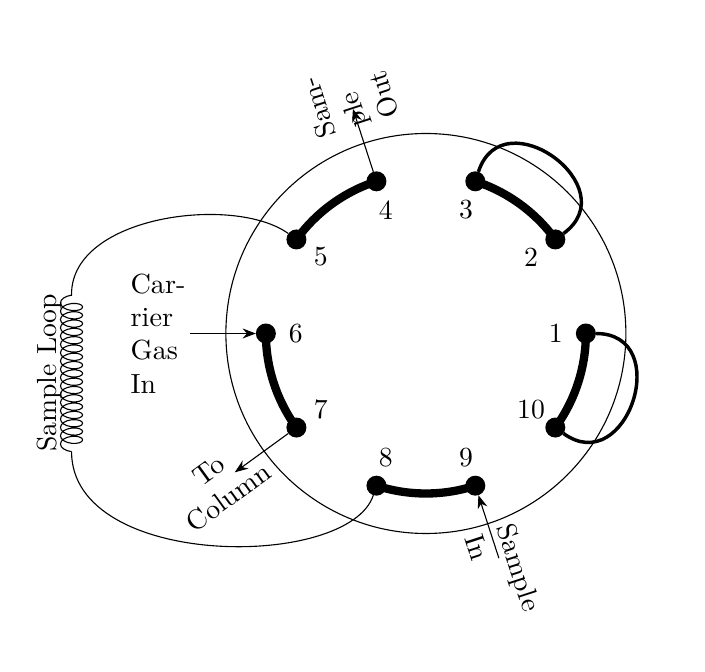
\begin{tikzpicture}
\draw (0,0) circle [radius=1in];
\fill (0,0) foreach \i / \j in {0/1,36/2,72/3,108/4,144/5,180/6,216/7,252/8,288/9,324/10}
     {+(\i:0.8in) circle [radius=0.05in] node at +(\i:0.65in) {\j}};
\draw[line width=3pt] +(0:0.8in) arc [start angle=0, end angle=-36, radius=0.8in];
\draw[line width=3pt] +(72:0.8in) arc [start angle=72, end angle=36, radius=0.8in];
\draw[line width=3pt] +(144:0.8in) arc [start angle=144, end angle=108, radius=0.8in];
\draw[line width=3pt] +(216:0.8in) arc [start angle=216, end angle=180, radius=0.8in];
\draw[line width=3pt] +(288:0.8in) arc [start angle=288, end angle=252, radius=0.8in];
\draw[Stealth-] +(180:0.85in) -- ++(180:3) node[text width = 1cm] at +(180:0.25) {Carrier Gas In};
\draw[-Stealth] +(216:0.85in) -- ++(216:3) node[rotate = 36, text width = 1.25cm, align=center] at +(216:0.25) {To \\ Column};
\draw +(252:0.85in) ..controls +(252:1) and +(90:-1.5).. (-4.5,-1.5);
\draw[decorate, decoration={coil,amplitude=4pt,segment length=3pt}]
    (-4.5,-1.5) -- (-4.5,0.5) node[midway,above,rotate=90] {Sample Loop};
\draw (-4.5,0.5) ..controls +(90:1) and (144:3).. (144:0.85in);
\draw[Stealth-] +(288:0.85in) -- ++(288:3) node[rotate = 288,text width=1.25cm] at +(288:0.25) {Sample In};
\draw[-Stealth] +(108:0.85in) -- ++(108:3) node[rotate=108, text width = 1cm] at +(108:0.25) {Sample Out};
\draw[line width=1.25pt] +(72:0.85in) ..controls +(72:1) and +(36:1).. +(36:0.85in);
\draw[line width=1.25pt] +(0:0.85in) ..controls +(0:1) and +(324:1).. +(324:0.85in);
\end{tikzpicture}
\end{document}